\documentclass[note=hide]{beamer} %für die Präsentation
%\documentclass[note=hide,handout]{beamer} %zum Drucken

\usepackage[ngerman]{babel}
\usepackage[latin1,utf8]{inputenx}
\usepackage[T1]{fontenc}
\usepackage{lmodern}

\usetheme{heidelberg}
%\usetheme{Malmoe}
%\usecolortheme{seahorse}
%\useoutertheme{smoothbars}

\usepackage{floatflt}
\usepackage{graphicx}
\usepackage{hyperref}
\usepackage{color}

%\usepackage{verbatim}
%\usepackage{moreverb}
%\usepackage{alltt}

%\usepackage{comment}
\usepackage{booktabs}
%\usepackage{rotating}
%\usepackage{fixltx2e}
%\usepackage{tikz}
%\usetikzlibrary{positioning,shadows,shapes,arrows}
% color definitions
\definecolor{dunkelrot}{RGB}{139, 0, 0} 
\definecolor{dunkelgruen}{RGB}{0,100,0}

\usepackage{listings} %für Code-Fragmente
\lstset{
   basicstyle=\ttfamily\scriptsize\mdseries,
   keywordstyle=\bfseries\color[rgb]{0,0,1},
   identifierstyle=,
   commentstyle=\color[rgb]{0,0.58,0},  
   stringstyle=\itshape\color[rgb]{0.65,0.16,0},
   numbers=left,
   numberstyle=\tiny,
   stepnumber=1,
   breaklines=true,
   frame=none,
   showstringspaces=false,
   tabsize=4,
   backgroundcolor=\color[rgb]{0.9,0.9,0.9},
   captionpos=b,
   float=htbp,
   language=Matlab,
   xleftmargin=15pt,
   xrightmargin=15pt
} 
%Beispiele
%-> \begin{lstlisting}[language=JAVA,firstnumber=27] ... \end{lstlisting}
%-> \lstinline[language=JAVA]{...}
%-> for beamer, embed it in a fragile frame!: \begin{frame}[fragile]{Beispiel} ... \end{frame}

%%%%%%%%% Our additions %%%%%%%%%%

\usepackage{siunitx}
\usepackage{adjustbox}

\definecolor{unirot}{rgb}{0.5976525,0,0}
\setbeamercolor{alerted text}{fg=unirot}

\AtBeginSection[]
{
	\begin{frame}
		\frametitle{Gliederung}
		\tableofcontents[currentsection]
	\end{frame}
}

\newcommand{\pymodule}[1]{\texttt{#1}}
\newcommand{\proglang}[1]{\texttt{#1}}
\newcommand{\feature}[1]{\textcolor{dunkelrot}{\emph{#1}}}
\newcommand{\ellipse}{[\ldots]}
\newcommand{\checkthis}[1]{#1}

\title[vilperg-senti]{Sentimentanalyse auf Amazon-Reviews}
%\subtitle{<Referatstitel> \\ -- Referat -- }
\author[berg, will]{Caroline Berg \\ Simon Will}
\institute[]{Institut für Computerlinguistik 
	\\ Ruprecht-Karls-Universität Heidelberg
	\\ Dozentin: Éva Mújdricza-Maydt
	\\ WS 2015/2016}
\date{3. Februar 2016}

\begin{document}

\begin{frame}[plain]
	\titlepage
\end{frame}

\begin{frame}{Gliederung}
	\tableofcontents
\end{frame}


\section{Überblick}

\begin{frame}{Einführung} % text aligned in the middle
	\begin{itemize}
		\item Unser Projekt: Sentimentanalyse auf Amazon-Reviews\\[0.3cm]
			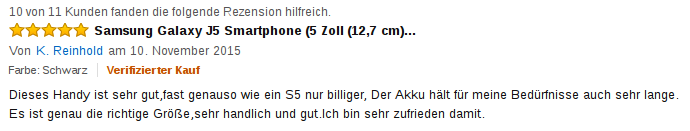
\includegraphics[width=\textwidth]{amazon_review_galaxy.png}
		\item Ziel: Anzahl der für ein Produkt vergebenen Sterne (1--5) aus dem Reviewtext vorhersagen
		\item Für einen Teil der Auswertung wurden die fünf Klassen binarisiert zu \emph{gut} und \emph{schlecht}.
	\end{itemize}
\end{frame}

\begin{frame}{Vergleichbare Projekte} %text always begins on top
	\begin{itemize}
		\item Callen \textsc{Rain}: Sentiment Analyses in Amazon Reviews Using Probabilistic Machine Learning.
		\item Reviews aus Büchern, Filmen, CDs, \ldots
		\item Klassifizierung:
		\begin{itemize}
			\item 1--2 Sterne: score 0
			\item 5 Sterne: score 1
		\end{itemize}
	\end{itemize}
\end{frame}

\begin{frame}{Vergleichbare Projekte}
	\begin{itemize}
		\item Feature-Extraction bei \textsc{Rain}
		\begin{itemize}
			%\item \feature{bag of words}: 2000 häufigste Wörter in Reviews (0 für ja, 1 für nein)
			\item \feature{bag of words}: Vorkommen der 2000 häufigsten Wörter in Reviews (binär)
			\item \feature{collocations}: \emph{bigram function} von NLTK (500 häufigste Bigramme, analog zu bag of words)
			\item \feature{negation}: nach einer Negation werden die drei darauffolgenden Wörter mit \emph{(NOT)} annotiert
			\item \feature{sentence length}: 
			\begin{itemize}
				\item sentence feature für kurze Sätze ($<10$)
				\item sentence feature für lange Sätze ($>20$)
			\end{itemize}
		\item Ergebnisse (Accuracy):
			\begin{itemize}
				\item Amazon Kindle (Naive Bayes): \SI{84}{\%}
				\item MacBook (Naive Bayes): \SI{88.2}{\%}
			\end{itemize}
		\end{itemize}
	\end{itemize}
\end{frame}

\section{Projektablauf}

\begin{frame}{Flussdiagramm}
	\begin{center}
	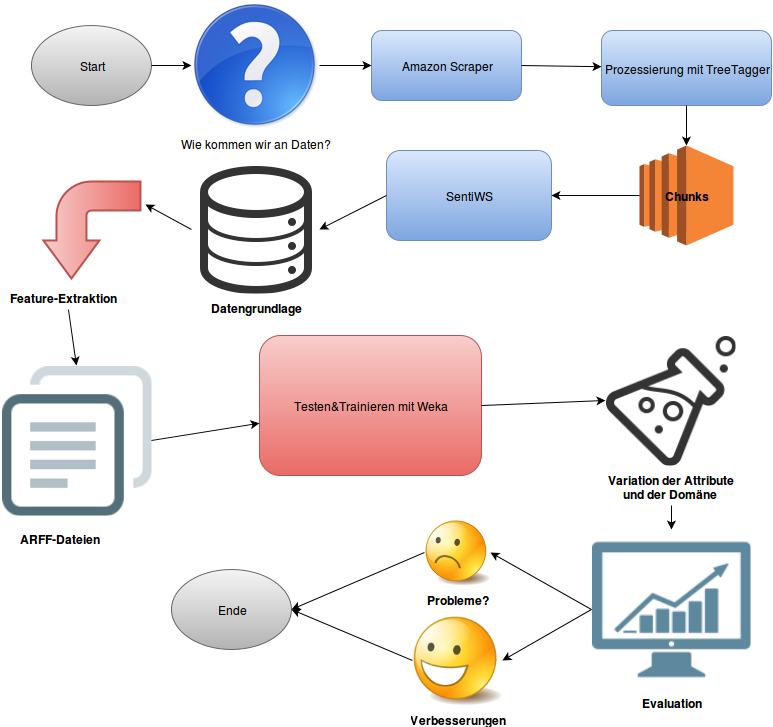
\includegraphics[scale=0.287]{flussdiagramm.png}
	\end{center}
\end{frame}

\begin{frame}{Amazon Scraper}
	\begin{itemize}
		\item geschrieben in \proglang{python3} mit \pymodule{urllib2}, \pymodule{BeautifulSoup} und \pymodule{lxml}
		\item ruft eine Überblicksseite auf Amazon auf, auf der Produkte aufgelistet sind und lädt alle Reviews herunter.\\[0.3cm]
			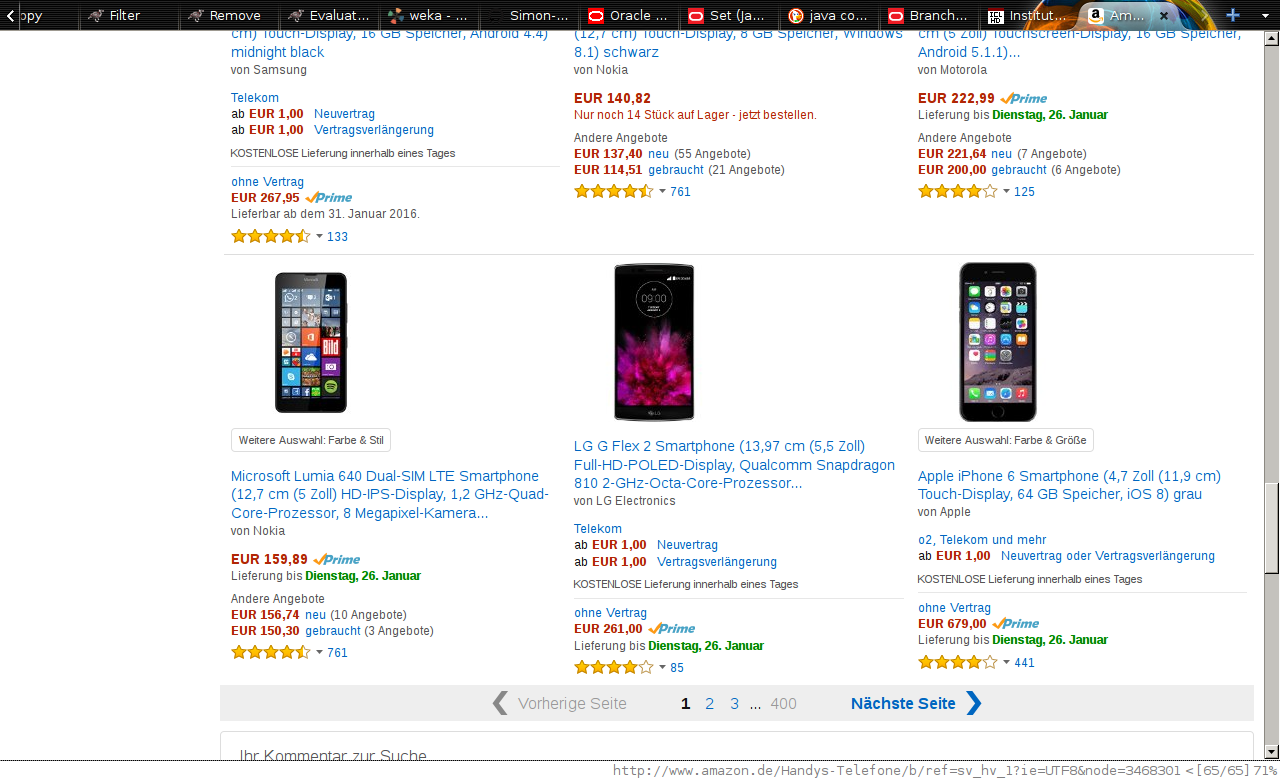
\includegraphics[height=0.6\textheight]{amazon_overview_smartphones.png}
		\item ruft dann die nächste Überblicksseite auf usw.
	\end{itemize}
\end{frame}

\begin{frame}[fragile]{Vorverarbeitung}
	\begin{itemize}
		\item Mit dem TreeTagger und den mit ihm gelieferten Skripten wurden die Reviews
			\begin{itemize}
				\item tokenisiert,
				\item mit POS-Tags versehen und
				\item lemmatisiert. \\[0.3cm]
			\end{itemize}
	\end{itemize}
	%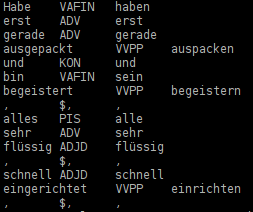
\includegraphics[width=0.8\textwidth]{content_tagged_example_black.png}
	\lstinputlisting[lastline=15]{content_tagged_example.txt}
\end{frame}

\begin{frame}{Einteilung in Chunks}
	Sternverteilung der Smartphone-Reviews:
	\begin{center}
		\renewcommand{\arraystretch}{1.3}
		\begin{tabular}{l|*{5}{c}|c}
			Sterne & $1$ & $2$ & $3$ & $4$ & $5$ & Gesamt \\
			\hline
			Anzahl & $13231$ & $6645$ & $8794$ & $21826$ & $77310$ & $127806$ \\
		\end{tabular}
	\end{center}
	\vspace{0.3cm}
	$\Rightarrow$ Eine Ausbalancierung ist nötig.\\[0.3cm]
	\begin{itemize}
		\item Erstellung einer Struktur aus symbolischen Links
		\item Jeder Symlink zeigt zufällig auf ein Review.
		\item Anordnung der Symlinks in balancierten Verzeichnissen (\emph{Chunks})
		\item geschrieben in \proglang{perl5}
		\item noch $33500$ Reviews nach dem Ausbalancieren übrig
	\end{itemize}
\end{frame}

\begin{frame}{Einteilung in Chunks}
	\begin{center}
		\includegraphics[scale=0.33]{chunks_diagram.png}
	\end{center}
\end{frame}

\begin{frame}{Ressource: SentiWS}
	\begin{itemize}
		\item \emph{SentiWS} (kurz für ,,Sentimentwortschatz``) ist eine Datenbank, die deutschen Wörtern Zahlen von $-1$ bis $1$ zuordnet, die das \checkthis{Sentiment} der Wörter darstellen soll.
		\item Enthalten sind etwa $33000$ Wortformen zu etwa $3500$ Lemmata.
	\end{itemize}
	%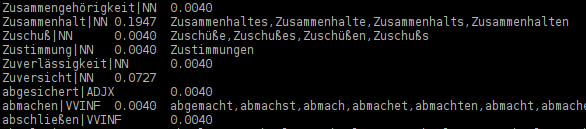
\includegraphics[width=\textwidth]{sentiws_example_black.png}
	{
		% lstinputlisting kommt nicht mit Zeichen klar, die durch mehr als ein Byte kodiert sind.
		% Daher wird der Text im Encoding ISO-8859-1 gespeichert.
		% Allerdings muss dafür in LaTeX das InputEncoding geändert werden.
		\InputEncoding{latin1}
		\lstinputlisting{sentiws_example_latin1.txt}
	}
\end{frame}

\begin{frame}{Feature-Extraktion}
	\begin{itemize}
		\item geschrieben in \proglang{python3} (und \proglang{sh}, \proglang{bash} und \proglang{awk})
		\item Attribute: \feature{token\_number}, \feature{overall\_sentiment}, \feature{adjective\_sentiment}, \feature{noun\_sentiment}, \feature{verb\_sentiment}
		\item Die Sentiment-Attribute existieren auch in einer auf die \feature{token\_number} normierten Version.\footnote{$\text{normalized\_overall\_sentiment} = \frac{\text{overall\_sentiment} * 10^6}{\text{token\_number}}$}
		\item Klassenattribute: \feature{stars} und \feature{binary\_judgement}
	\end{itemize}
	%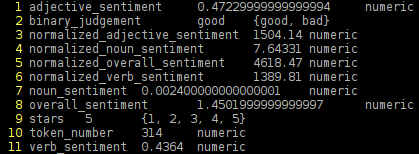
\includegraphics[width=\textwidth]{features_example_black.png}
	\lstinputlisting{features_example.txt}
\end{frame}

\begin{frame}{ARFF-Datei}
	%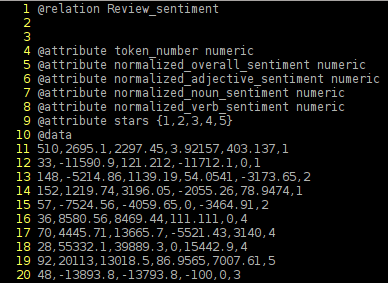
\includegraphics[width=\textwidth]{arff_example_black.png}
	\lstinputlisting{arff_example.txt}
\end{frame}

\section{Evaluation und Experimente}

\begin{frame}{Benutzte Klassifizierer}
	\begin{itemize}
		\item J48 mit 
			\begin{description}
				\item[-U] ,,Use unpruned tree``
			\end{description}
		\item RandomForest mit 
			\begin{description}
				\item[-I 10] ,,Number of trees to build``
				\item[-K 0] ,,Number of features to consider``
				\item[-S 1] ,,Seed for random number generator``
				\item[-depth 200] ,,The maximum depth of the trees``
			\end{description}
		\item NaiveBayes ohne Optionen
	\end{itemize}
\end{frame}

\begin{frame}{Hauptsächliche Ergebnisse}

	Mit zehnfacher Kreuzvalidierung ergeben sich folgende Ergebnisse:

	\adjustbox{max width=\textwidth,vspace=3ex}
	{
		\begin{tabular}{lccccc}
			\toprule
			Klassen & normiert & Majority Voting & J48 & RandomForest & Naive Bayes \\
			\midrule
			1--5 & nein & \SI{20}{\%} &\SI{61.0}{\%} & \SI{67.4}{\%} & \SI{31.6}{\%} \\
			1--5 & ja & \SI{20}{\%} &\SI{61.0}{\%} & \alert{\SI{67.6}{\%}} & \SI{32.5}{\%} \\
			binär & ja & \SI{60}{\%} & \SI{75.0}{\%} & \SI{84.6}{\%} & \SI{69.8}{\%} \\
			\bottomrule
		\end{tabular}
	}
	Wird ein Teil der Daten eigens zum Testen abgetrennt, verringert sich die Accuracy etwas (von \SI{67.6}{\%} beim RandomForest auf \SI{64.7}{\%}).
	Das liegt wohl einfach daran, dass dann auf weniger Daten trainiert wird.
	
\end{frame}

\begin{frame}{Variieren der Trainingsdatenmenge}
	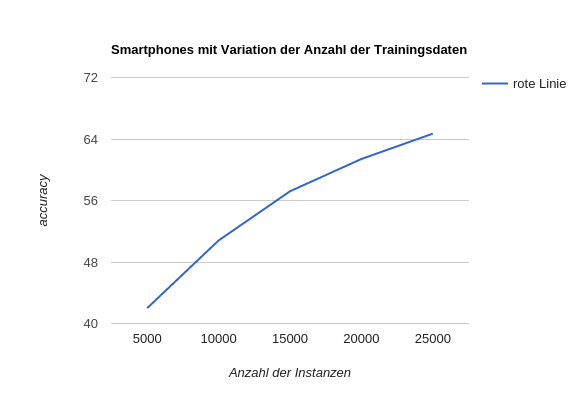
\includegraphics[width=\framewidth]{accuracy_smartphones_normalized_trainsize.png}
\end{frame}

\begin{frame}{Attributselektion}
	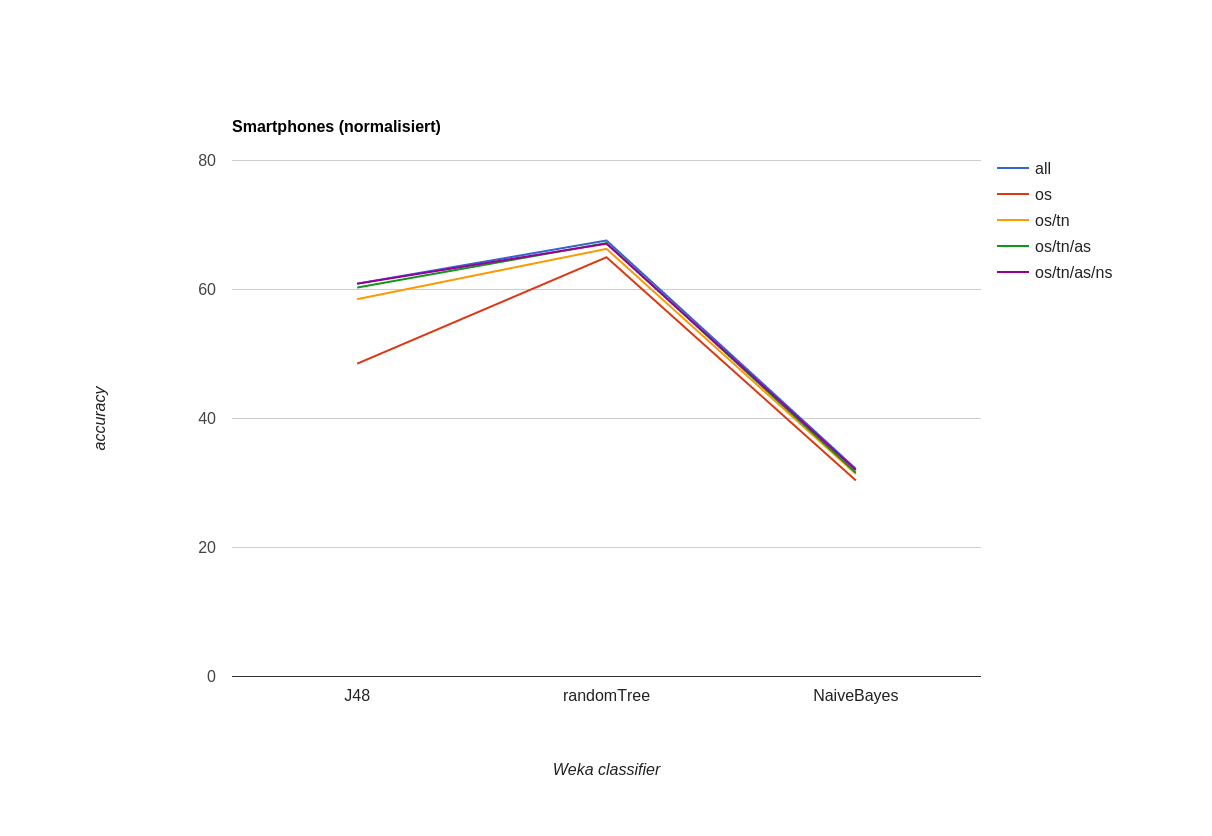
\includegraphics[width=\framewidth]{accuracy_smartphones_normalized.png}
\end{frame}

\begin{frame}{Test auf fremder Domäne}

	\begin{itemize}
		\item Test des mit den normierten Sentimentattributen und \feature{token\_number} auf Smartphones trainierten Modells auf Armbanduhren
		\item Erreichte Accuracy: \SI{27.7}{\%}
		\item Ein Faktor eventuell: Armbanduhren-Reviews sind nur etwa ein Drittel so lang wie Smartphone-Reviews.
	\end{itemize}
\end{frame}

\begin{frame}{Fehlersuche}
	\begin{block}{Review mit 5 Sternen}
		\it
		Super Handy, Habe mir dieses Handy bestellt, weil wir schon das gleiche in der Familie haben. Einfache Bedienung, tolle Menüführung. Einfach Klasse für einen guten Preis.
	\end{block}
\end{frame}

\begin{frame}{Fehlersuche}
	\begin{block}{Review mit 5 Sternen}
		\it
	Ich persönlich komme vom Nokia E51 :) und habe über nun fast ein halbes Jahr verschiedene Smartphones \ellipse\ begutachtet. Ebenfalls im Focus hatte ich (Nachteile ggü. dem S3 hier aufgeführt): Motorola RAZR MAXX: kein Wechselakku, Andoid 4.1 ungewiß; HTC One X: kein Wechselakku, kein Glonass, kein SD-SchachtSamsung Galaxy Note: schlechtere Performance, Andoid 4.1 ungewiß; Samsung Galaxy Ace 2: schlechtere Performance, wenig Flashspeicher, Andoid 4.1 ungewiß; Meine Eindrücke \ellipse\ des S3 kurz zusammengefasst:positiv:- Display: hohe Auflösung, schöne Farben, die Größe möchte ich wirklich nicht mehr missen \ellipse
	\end{block}
\end{frame}

\begin{frame}{Schluss}

	\begin{itemize}
		\item Überraschend gute Ergebnisse für den naiven Ansatz.
		\item Weitere mögliche Schritte:
			\begin{itemize}
				\item Einbezug von Texstruktur
				\item Einbezug von Negation und anderen privativen Ausdrücken
			\end{itemize}
		\item Problem: Textgattung ,,Amazon-Review`` nicht sehr einheitlich
	\end{itemize}
\end{frame}

\begin{frame}{Literatur}
	\small
	\textsc{Rain,} Callen: \textit{Sentiment Analysis in Amazon Reviews Using Probabilistic Machine Learning.} Swarthmore : Department of Computer Science, Swarthmore College, 2013.\\[0.3cm]

	\textsc{Remus,} R.; \textsc{Quasthoff,} U.; \textsc{Heyer,} G.: \textit{SentiWS -- a Publicly Available German-language Resource for Sentiment Analysis.} In: \textit{Proceedings of the 7th International Language Ressources and Evaluation (LREC'10),} Valetta : 2010, S. 1168--1171.\\[0.3cm]

	\textsc{Schmid,} Helmut.: \textit{Probabilistic Part-of-Speech Tagging Using Decision Trees.} In: \textit{Proceedings of International Conference on New Methods in Language Processing,} Manchester : 1994.
\end{frame}

\end{document}
